% Common patterns: graphical linear algebra, the linear algebra course,
% category theory --- and tilings as a device for reasoning.
% Compile with:  tectonic patterns.tex   (or pdflatex patterns.tex, twice)
\documentclass[11pt]{article}
\usepackage[T1]{fontenc}
\usepackage[a4paper,margin=25mm]{geometry}
\usepackage{lmodern}
\usepackage{amsmath,amssymb,amsthm}
\usepackage{tikz}
\usetikzlibrary{calc,positioning,arrows.meta,decorations.pathmorphing,fit,backgrounds,shapes.geometric,patterns}
\usepackage{booktabs}
\usepackage{longtable}
\usepackage{hyperref}
\hypersetup{colorlinks=true,linkcolor=blue!50!black,urlcolor=blue!50!black}

\theoremstyle{definition}
\newtheorem{definition}{Definition}[section]
\theoremstyle{plain}
\newtheorem{theorem}[definition]{Theorem}
\newtheorem{lemma}[definition]{Lemma}
\newtheorem{proposition}[definition]{Proposition}
\newtheorem{corollary}[definition]{Corollary}
\theoremstyle{remark}
\newtheorem{remark}[definition]{Remark}
\newtheorem{exercise}[definition]{Exam pattern}

\newcommand{\lean}[1]{\texttt{\small #1}}
\newcommand{\file}[1]{\texttt{\small #1}}
\newcommand{\K}{\mathbb{K}}
\newcommand{\Z}{\mathbb{Z}}
\newcommand{\R}{\mathbb{R}}
\newcommand{\id}{\mathrm{id}}
\newcommand{\tr}{\operatorname{tr}}
\newcommand{\rank}{\operatorname{rank}}

\tikzset{
  wire/.style={line width=0.7pt},
  box/.style={draw, fill=white, minimum width=9mm, minimum height=8mm, inner sep=2pt},
  smallbox/.style={draw, fill=white, minimum width=7mm, minimum height=6mm, inner sep=1pt},
  bdot/.style={circle, draw, fill=black, inner sep=0pt, minimum size=4.5pt},
  wdot/.style={circle, draw, fill=white, inner sep=0pt, minimum size=4.5pt},
  tile/.style={draw=black, line width=0.5pt},
  every picture/.append style={baseline=(current bounding box.center)}
}

\title{\bf Common patterns\\[2mm]
\large Graphical linear algebra, the linear algebra course, and category
theory --- and how to reason with tilings\\ (with machine-checked proofs in Lean~4)}
\author{}
\date{}

\begin{document}
\sloppy
\maketitle

\begin{abstract}
Three things that look different --- the circuit diagrams of graphical linear
algebra, the theorems of an undergraduate linear algebra course, and the arrows
of category theory --- are three dialects of one grammar.  This note isolates
the eight patterns they share, draws each of them, and points at the Lean
theorem that proves it.  It then does the same for a fourth dialect that is
rarely put next to the others: \emph{tilings and patterns}.  Drawing a tiling is
a legitimate way to reason about determinants, change of basis, Gaussian
elimination, solution sets, rank and symmetry, and the last two sections
collect the exam patterns and the big ideas that come out of it.  Every picture
in this note is backed by a theorem in the companion Lean~4 development in
\file{RequestProject/}, which builds against Mathlib with no \lean{sorry} and no
added axioms.  The two new modules are \file{RequestProject/CommonPatterns.lean}
(the eight patterns) and \file{RequestProject/Tilings.lean} (the tiling
material, up to the crystallographic restriction).
\end{abstract}

\tableofcontents

\section{One grammar, three dialects}

A linear algebra course, a category theory course and the string-diagram
calculus of graphical linear algebra all spend their time on the same short list
of facts.  They differ only in what they draw.

\begin{center}
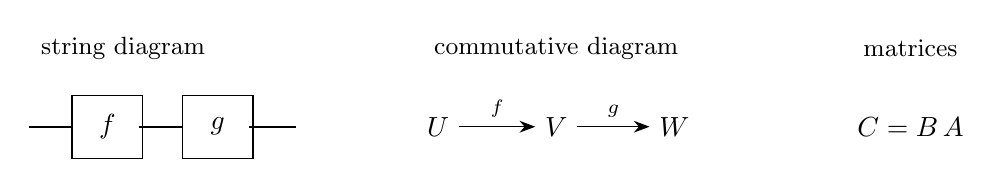
\begin{tikzpicture}[x=1mm,y=1mm]
  % string diagram
  \node at (0,18) {\small string diagram};
  \draw[wire] (-12,8) -- (-6,8);
  \node[box] (f) at (-2,8) {$f$};
  \draw[wire] (2,8) -- (8,8);
  \node[box] (g) at (12,8) {$g$};
  \draw[wire] (16,8) -- (22,8);
  % arrows
  \node at (55,18) {\small commutative diagram};
  \node (A) at (40,8) {$U$};
  \node (B) at (55,8) {$V$};
  \node (C) at (70,8) {$W$};
  \draw[-{Stealth[length=2mm]}] (A) -- node[above,font=\scriptsize]{$f$} (B);
  \draw[-{Stealth[length=2mm]}] (B) -- node[above,font=\scriptsize]{$g$} (C);
  % matrices
  \node at (100,18) {\small matrices};
  \node at (100,8) {$C = B\,A$};
\end{tikzpicture}
\end{center}

\noindent
The dictionary is the following.  Each row is proved, in the stated generality,
in the file \file{CommonPatterns.lean}.

\begin{center}\small
\begin{tabular}{@{}p{25mm}p{29mm}p{33mm}p{40mm}@{}}
\toprule
\textbf{pattern} & \textbf{picture} & \textbf{textbook} & \textbf{Lean} \\
\midrule
composition & wires plug together & $(AB)C=A(BC)$, $IA=A$ & \lean{series\_assoc}, \lean{bare\_wire\_left} \\
functor & read a picture as a matrix & the matrix of a composite is the product & \lean{toMatrix\_series} \\
interchange & a picture has no reading order & $(A\otimes B)(C\otimes D)=AC\otimes BD$ & \lean{interchange\_kronecker} \\
universal property & a box with a unique filler & extend a map linearly from a basis & \lean{unique\_extension\_}\newline\lean{from\_basis} \\
duality & bend a wire & $\langle Ax,y\rangle=\langle x,A^{\!\top}y\rangle$ & \lean{bend\_wire}, \lean{bend\_series} \\
partition & cut a wire into strands & $A=\sum_{ij}a_{ij}E_{ij}$ & \lean{identity\_is\_tiled}, \lean{matrix\_is\_tiled} \\
change of coordinates & redraw with new labels & similar matrices & \lean{change\_of\_basis} \\
fibration & tile the domain in slices & solution $=$ particular $+$ kernel & \lean{fibre\_eq\_kernel\_}\newline\lean{translate} \\
\bottomrule
\end{tabular}
\end{center}

\section{The eight patterns, drawn}

\subsection{Pattern 1: composition (the category pattern)}

Plugging wires end to end is associative, and a bare wire changes nothing.  In a
picture there are no brackets, which is exactly why nobody writes them.

\begin{center}
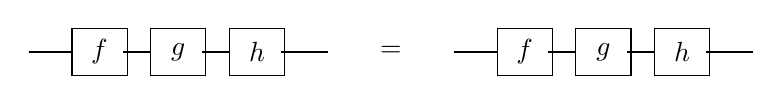
\begin{tikzpicture}[x=1mm,y=1mm]
  \draw[wire] (-14,0) -- (-8,0);
  \node[smallbox] at (-5,0) {$f$};
  \draw[wire] (-2,0) -- (2,0);
  \node[smallbox] at (5,0) {$g$};
  \draw[wire] (8,0) -- (12,0);
  \node[smallbox] at (15,0) {$h$};
  \draw[wire] (18,0) -- (24,0);
  \node at (32,0) {$=$};
  \draw[wire] (40,0) -- (46,0);
  \node[smallbox] at (49,0) {$f$};
  \draw[wire] (52,0) -- (56,0);
  \node[smallbox] at (59,0) {$g$};
  \draw[wire] (62,0) -- (66,0);
  \node[smallbox] at (69,0) {$h$};
  \draw[wire] (72,0) -- (78,0);
\end{tikzpicture}
\end{center}

\noindent
\emph{Category theory:} this is the definition of a category.  \emph{Textbook:}
associativity of the matrix product, proved by exchanging two summation signs
(\lean{matrix\_series\_assoc}, and entry by entry in
\file{SzaboMatrices.lean}).  \emph{Graphical linear algebra:} the fact that a
diagram is a graph, not a term.

\subsection{Pattern 2: functor (choosing a basis)}

A basis turns a linear map into a matrix, and it does so \emph{compatibly} with
composition and identities.  That compatibility is the single fact that makes
matrix computations legitimate.
\[
  \big[g\circ f\big]_{b}^{d} \;=\; [g]_{c}^{d}\,[f]_{b}^{c},
  \qquad [\id]_b^b = I .
\]
Lean: \lean{toMatrix\_series}, \lean{toMatrix\_bare\_wire}.

\subsection{Pattern 3: interchange (a diagram has no reading order)}

Two boxes drawn side by side may be composed first horizontally or first
vertically; the results agree.

\begin{center}
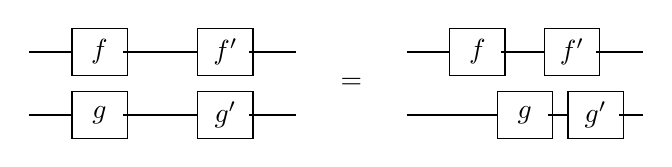
\begin{tikzpicture}[x=1mm,y=1mm]
  \draw[wire] (-14,4) -- (-8,4); \node[smallbox] at (-5,4) {$f$}; \draw[wire] (-2,4) -- (4,4);
  \draw[wire] (-14,-4) -- (-8,-4); \node[smallbox] at (-5,-4) {$g$}; \draw[wire] (-2,-4) -- (4,-4);
  \draw[wire] (4,4) -- (8,4); \node[smallbox] at (11,4) {$f'$}; \draw[wire] (14,4) -- (20,4);
  \draw[wire] (4,-4) -- (8,-4); \node[smallbox] at (11,-4) {$g'$}; \draw[wire] (14,-4) -- (20,-4);
  \node at (27,0) {$=$};
  \draw[wire] (34,4) -- (40,4); \node[smallbox] at (43,4) {$f$}; \draw[wire] (46,4) -- (52,4);
  \node[smallbox] at (55,4) {$f'$}; \draw[wire] (58,4) -- (64,4);
  \draw[wire] (34,-4) -- (46,-4); \node[smallbox] at (49,-4) {$g$}; \draw[wire] (52,-4) -- (55,-4);
  \node[smallbox] at (58,-4) {$g'$}; \draw[wire] (61,-4) -- (64,-4);
\end{tikzpicture}
\end{center}

\noindent
\emph{Category theory:} $\otimes$ (or $\oplus$) is a bifunctor.
\emph{Textbook:} the mixed product rule $(A\otimes A')(B\otimes B') = AB \otimes
A'B'$ for Kronecker products.  \emph{Lean:} \lean{interchange\_prod},
\lean{interchange\_kronecker}, \lean{slide\_past\_wire}.

\subsection{Pattern 4: universal property (say it on generators)}

\begin{center}
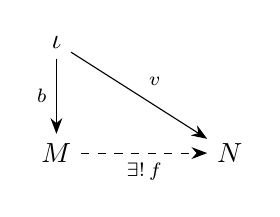
\begin{tikzpicture}[x=1mm,y=1mm]
  \node (I) at (0,10) {$\iota$};
  \node (M) at (0,-4) {$M$};
  \node (N) at (22,-4) {$N$};
  \draw[-{Stealth[length=2mm]}] (I) -- node[left,font=\scriptsize]{$b$} (M);
  \draw[-{Stealth[length=2mm]}] (I) -- node[above right,font=\scriptsize]{$v$} (N);
  \draw[-{Stealth[length=2mm]},dashed] (M) -- node[below,font=\scriptsize]{$\exists!\,f$} (N);
\end{tikzpicture}
\end{center}

\noindent
Every ``define a linear map by prescribing its values on a basis'' exercise is
this triangle: the free module on the index set.  Uniqueness is what lets a
diagrammatic law be checked on generators only.  Lean:
\lean{unique\_extension\_from\_basis}, \lean{eq\_of\_eq\_on\_basis}.

\subsection{Pattern 5: duality (bending a wire)}

\begin{center}
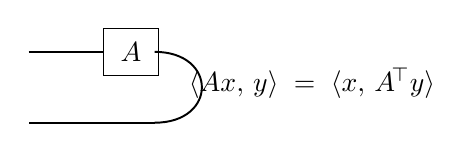
\begin{tikzpicture}[x=1mm,y=1mm]
  \draw[wire] (-16,3) -- (-6,3);
  \node[smallbox] at (-3,3) {$A$};
  \draw[wire] (0,3) .. controls (8,3) and (8,-6) .. (0,-6);
  \draw[wire] (0,-6) -- (-16,-6);
  \node at (20,-1) {$\langle Ax,\,y\rangle \;=\; \langle x,\,A^{\!\top}y\rangle$};
\end{tikzpicture}
\end{center}

\noindent
\emph{Category theory:} compact closedness --- the cup and the cap and the two
snake equations.  \emph{Textbook:} the transpose is the adjoint of the dot
product, and $(AB)^{\!\top} = B^{\!\top}A^{\!\top}$ because bending reverses the
order.  \emph{Lean:} \lean{bend\_wire}, \lean{bend\_twice}, \lean{bend\_series}.

\subsection{Pattern 6: partition (cut a wire into strands)}

\[
  \sum_i E_{ii} = I, \qquad A = \sum_{i,j} a_{ij} E_{ij},
  \qquad x = \sum_j x_j e_j .
\]
This is already a tiling: the identity matrix is tiled by its diagonal cells and
an arbitrary matrix by its rank-one cells.  It is the computational content of
``choose a basis'', and in category theory it is a biproduct decomposition
$\id = \sum_i \iota_i\pi_i$.  Lean: \lean{identity\_is\_tiled},
\lean{matrix\_is\_tiled}, \lean{vector\_is\_tiled}.

\subsection{Pattern 7: change of coordinates}

Relabelling the wires conjugates the box: $[f]_{b}^{c} = P\,[f]_{b'}^{c'}Q$ with
$P,Q$ the transition matrices (\lean{change\_of\_basis}), and in the square case
$B = X^{-1}AX$.  Everything that survives conjugation --- rank, trace,
determinant, characteristic polynomial --- is a property of the \emph{picture}
rather than of the coordinates; see \file{trace-loop.pdf} and
\file{RequestProject/TraceLoop.lean} for the trace, where the invariance is the
statement that a box may be slid around a closed loop.

\subsection{Pattern 8: fibration (tile the domain)}

\begin{center}
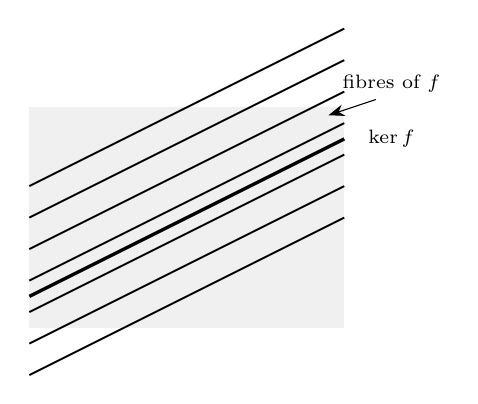
\begin{tikzpicture}[x=1mm,y=1mm]
  \fill[gray!12] (-20,-14) rectangle (20,14);
  \foreach \s in {-12,-8,-4,0,4,8,12}{
    \draw[wire] (-20,\s-8) -- (20,\s+12);
  }
  \draw[very thick] (-20,-10) -- (20,10);
  \node[font=\scriptsize] at (26,10) {$\ker f$};
  \node[font=\scriptsize] at (26,17) {fibres of $f$};
  \draw[-{Stealth[length=2mm]}] (24,15) -- (18,13);
\end{tikzpicture}
\end{center}

\noindent
The fibres $\{x : f(x) = c\}$ are the translates of $\ker f$: parallel tiles,
one for each point of the image.  Rank--nullity is the bookkeeping
``(number of tiles) $\times$ (size of a tile) $=$ size of the domain'':
\[
  \dim \operatorname{im} f + \dim \ker f = \dim V .
\]
Lean: \lean{fibre\_eq\_kernel\_translate}, \lean{fibres\_disjoint\_or\_equal},
\lean{fibres\_cover}, \lean{tiles\_times\_tile}, \lean{solution\_set\_is\_a\_tile}.

\section{Tilings and patterns as a reasoning device}

Grünbaum and Shephard's vocabulary translates into linear algebra almost word
for word.

\begin{center}\small
\begin{tabular}{@{}p{40mm}p{45mm}p{50mm}@{}}
\toprule
\textbf{tiling} & \textbf{linear algebra} & \textbf{Lean} \\
\midrule
prototile & fundamental parallelogram of a basis & \lean{ZSpan.fundamentalDomain} \\
the tiling (covers, no overlap) & every vector has unique coordinates mod the lattice & \lean{plane\_is\_tiled\_by\_lattice} \\
area of the prototile & $|\det|$ & \lean{tile\_area\_eq\_abs\_det} \\
re-tiling by a map & image of a set under a linear map & \lean{area\_scales\_by\_det} \\
shearing a tile & elementary row operation & \lean{shear\_preserves\_area} \\
degenerate (flat) tile & singular matrix & \lean{degenerate\_no\_tiling} \\
striped tiling by parallel lines & fibres of a linear map & \lean{fibre\_eq\_kernel\_translate} \\
symmetry group of the pattern & matrices preserving the lattice & \lean{lattice\_isometry\_cases} \\
admissible rotation orders & $1,2,3,4,6$ & \lean{pow\_twelve\_eq\_one} \\
\bottomrule
\end{tabular}
\end{center}

\subsection{A lattice tiles the plane; the tile has area $|\det|$}

\begin{center}
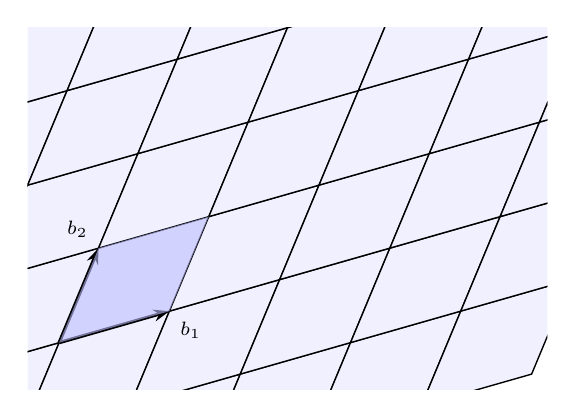
\begin{tikzpicture}[x=1mm,y=1mm]
  \clip (-4,-6) rectangle (62,40);
  \foreach \i in {-2,...,4}{
    \foreach \j in {-2,...,4}{
      \draw[tile,fill=blue!6]
        ($ \i*(14,4) + \j*(5,12) $) --
        ($ \i*(14,4) + \j*(5,12) + (14,4) $) --
        ($ \i*(14,4) + \j*(5,12) + (19,16) $) --
        ($ \i*(14,4) + \j*(5,12) + (5,12) $) -- cycle;
    }}
  \draw[-{Stealth[length=2mm]},very thick] (0,0) -- (14,4) node[below right,font=\scriptsize]{$b_1$};
  \draw[-{Stealth[length=2mm]},very thick] (0,0) -- (5,12) node[above left,font=\scriptsize]{$b_2$};
  \fill[blue!25,opacity=.6] (0,0) -- (14,4) -- (19,16) -- (5,12) -- cycle;
\end{tikzpicture}
\end{center}

Formally: for a basis $b$ of $\R^n$, every $x$ lies in exactly one translate
$v + D$, $v$ in the lattice $\Z b_1 + \dots + \Z b_n$, where
$D = \{\sum t_ib_i : 0 \le t_i < 1\}$ (\lean{plane\_is\_tiled\_by\_lattice}); all
tiles are translates, hence of equal area (\lean{tiles\_are\_congruent}); and
\[
  \operatorname{area}(D) = |\det(b_1,\dots,b_n)|
  \qquad\text{(\lean{tile\_area\_eq\_abs\_det})} ,
\]
which in the plane is the familiar $|ad-bc|$ (\lean{tile\_area\_fin\_two}).
\emph{This is the definition of the determinant that makes every determinant
exercise a picture.}

\subsection{A linear map re-tiles space}

If $f$ is linear then $\operatorname{vol}(f(S)) = |\det f| \cdot
\operatorname{vol}(S)$ for \emph{every} measurable $S$
(\lean{area\_scales\_by\_det}).  Two consequences that students are usually
asked to prove algebraically become one-line pictures.

\begin{center}
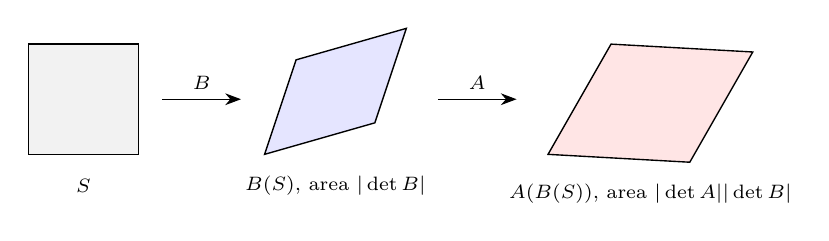
\begin{tikzpicture}[x=1mm,y=1mm]
  \draw[tile,fill=gray!10] (0,0) rectangle (14,14);
  \node[font=\scriptsize] at (7,-4) {$S$};
  \draw[-{Stealth[length=2mm]}] (17,7) -- node[above,font=\scriptsize]{$B$} (27,7);
  \draw[tile,fill=blue!10] (30,0) -- (44,4) -- (48,16) -- (34,12) -- cycle;
  \node[font=\scriptsize] at (39,-4) {$B(S)$, area $|\det B|$};
  \draw[-{Stealth[length=2mm]}] (52,7) -- node[above,font=\scriptsize]{$A$} (62,7);
  \draw[tile,fill=red!10] (66,0) -- (84,-1) -- (92,13) -- (74,14) -- cycle;
  \node[font=\scriptsize] at (79,-5) {$A(B(S))$, area $|\det A||\det B|$};
\end{tikzpicture}
\end{center}

\begin{enumerate}
\item $\det(AB) = \det A \cdot \det B$: re-tile twice
  (\lean{det\_mul\_is\_retiling}).
\item $\det A = 0$ iff the tile is flat, iff some nonzero vector is killed, iff
  the columns are dependent (\lean{degenerate\_no\_tiling}).
\end{enumerate}

\subsection{Gaussian elimination is a shear (Cavalieri's principle)}

Adding a multiple of one row to another slides the tile parallel to itself: same
base, same height, same area, so the determinant does not change.

\begin{center}
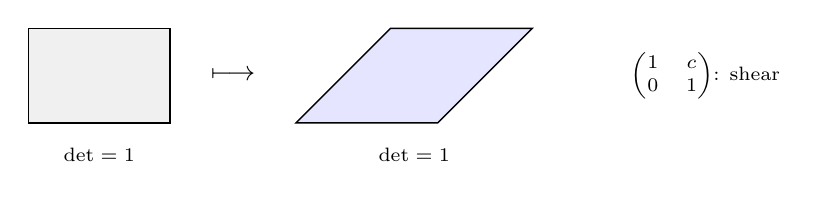
\begin{tikzpicture}[x=1mm,y=1mm]
  \draw[tile,fill=gray!12] (0,0) rectangle (18,12);
  \draw[dashed] (0,0) -- (18,0);
  \node[font=\scriptsize] at (9,-4) {$\det = 1$};
  \node at (26,6) {$\longmapsto$};
  \draw[tile,fill=blue!10] (34,0) -- (52,0) -- (64,12) -- (46,12) -- cycle;
  \draw[dashed] (34,0) -- (52,0);
  \node[font=\scriptsize] at (49,-4) {$\det = 1$};
  \node[font=\scriptsize] at (86,6) {$\begin{pmatrix}1&c\\0&1\end{pmatrix}$: shear};
\end{tikzpicture}
\end{center}

\noindent
Lean: \lean{row\_operation\_preserves\_det} (any size, any commutative ring) and
\lean{shear\_det}, \lean{shear\_preserves\_area} (the plane picture, with the
measure).  Swapping two rows reflects the tile ($\det \mapsto -\det$) and
scaling a row stretches it ($\det \mapsto \lambda\det$): the three elementary
operations are exactly the three ways of moving a tile.

\subsection{Change of basis re-tiles the same plane}

The \emph{same} lattice can be tiled by different prototiles of the same area;
the transition matrix is unimodular.  This is the picture behind ``similar
matrices are the same map in different coordinates''.

\begin{center}
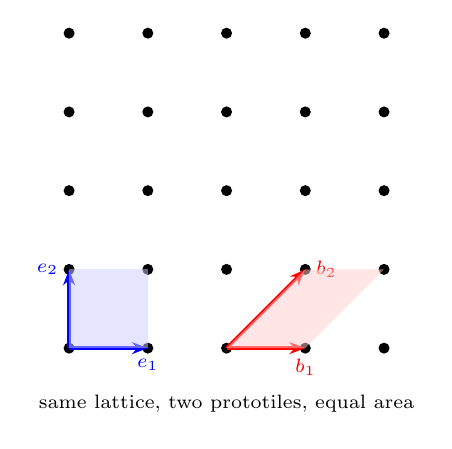
\begin{tikzpicture}[x=1mm,y=1mm]
  \foreach \i in {0,...,4}{\foreach \j in {0,...,4}{
    \fill (\i*10,\j*10) circle (0.7mm);}}
  \draw[-{Stealth[length=2mm]},very thick,blue] (0,0) -- (10,0) node[below,font=\scriptsize]{$e_1$};
  \draw[-{Stealth[length=2mm]},very thick,blue] (0,0) -- (0,10) node[left,font=\scriptsize]{$e_2$};
  \fill[blue!20,opacity=.5] (0,0) rectangle (10,10);
  \draw[-{Stealth[length=2mm]},very thick,red] (20,0) -- (30,0) node[below,font=\scriptsize]{$b_1$};
  \draw[-{Stealth[length=2mm]},very thick,red] (20,0) -- (30,10) node[right,font=\scriptsize]{$b_2$};
  \fill[red!20,opacity=.5] (20,0) -- (30,0) -- (40,10) -- (30,10) -- cycle;
  \node[font=\scriptsize] at (20,-7) {same lattice, two prototiles, equal area};
\end{tikzpicture}
\end{center}

\subsection{Symmetry: the crystallographic restriction}

A symmetry of a lattice, written in a lattice basis, is an \emph{integer}
matrix.  Its trace is therefore an integer.  A rotation by $\theta$ has trace
$2\cos\theta$, and $|2\cos\theta| \le 2$; hence
\[
  2\cos\theta \in \{-2,-1,0,1,2\},
  \qquad\text{so}\qquad
  \theta \in \Big\{\,\pi,\ \tfrac{2\pi}{3},\ \tfrac{\pi}{2},\ \tfrac{\pi}{3},\ 0 \,\Big\}.
\]
Only $1$-, $2$-, $3$-, $4$- and $6$-fold rotations preserve a lattice: there is
no fivefold wallpaper pattern.  This is a two-line linear algebra proof of a
theorem about tilings, and the whole of it is formalised
(\lean{two\_cos\_of\_lattice\_rotation}, \lean{cos\_of\_lattice\_rotation}).

\begin{center}
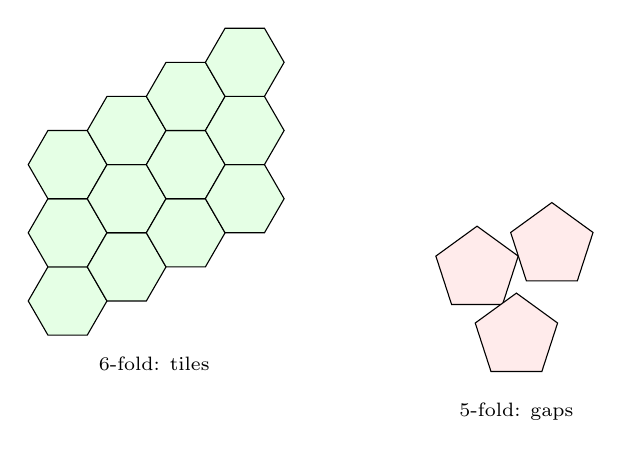
\begin{tikzpicture}[x=1mm,y=1mm]
  % hexagonal packing: works (flat-top honeycomb, circumradius 5mm)
  \foreach \i in {0,...,3}{\foreach \j in {0,...,2}{
    \draw[fill=green!10]
      ($ \i*(7.5,4.330) + \j*(0,8.660) + (0:5) $) --
      ($ \i*(7.5,4.330) + \j*(0,8.660) + (60:5) $) --
      ($ \i*(7.5,4.330) + \j*(0,8.660) + (120:5) $) --
      ($ \i*(7.5,4.330) + \j*(0,8.660) + (180:5) $) --
      ($ \i*(7.5,4.330) + \j*(0,8.660) + (240:5) $) --
      ($ \i*(7.5,4.330) + \j*(0,8.660) + (300:5) $) -- cycle;}}
  \node[font=\scriptsize] at (11,-8) {$6$-fold: tiles};
  % pentagons: fails
  \begin{scope}[xshift=52mm]
    \node[regular polygon, regular polygon sides=5, draw, minimum size=11mm, inner sep=0pt,
          fill=red!8] at (0,4) {};
    \node[regular polygon, regular polygon sides=5, draw, minimum size=11mm, inner sep=0pt,
          fill=red!8, rotate=72] at (9.5,7) {};
    \node[regular polygon, regular polygon sides=5, draw, minimum size=11mm, inner sep=0pt,
          fill=red!8, rotate=144] at (5,-4.5) {};
    \node[font=\scriptsize] at (5,-14) {$5$-fold: gaps};
  \end{scope}
\end{tikzpicture}
\end{center}

The algebraic version needs no geometry at all.  From the $2\times2$
Cayley--Hamilton identity $A^2 = (\tr A)A - (\det A)I$ one gets the recursion
$s_{k+2} = t\,s_{k+1} - s_k$ for $s_k = \tr(A^k)$, $t = \tr A$; if $t \ge 3$ the
$s_k$ increase strictly, so $A^n \ne I$ for all $n\ge1$
(\lean{no\_finite\_order\_of\_trace\_ge\_three}).  Applying this to $A$ and to
$-A$ gives $|\tr A|\le 2$ (\lean{abs\_trace\_le\_two}), and the five possible
traces give five possible minimal polynomials, whence
\[
  A^{12} = I \qquad \text{(\lean{pow\_twelve\_eq\_one})} .
\]
Two corollaries that are fun to state: \lean{no\_fivefold\_symmetry} (a
unimodular integer matrix with $A^5 = I$ is the identity) and
\lean{hexagonal\_rotation\_pow\_six} (the matrix
$\left(\begin{smallmatrix}0&-1\\1&1\end{smallmatrix}\right)$ has order exactly
$6$, so the bound is attained --- this is the $60^\circ$ rotation of the
triangular lattice written in the lattice basis).

\subsection{The point group of the square lattice}

Which integer matrices preserve lengths?  $A^{\!\top}A = I$ forces
$a^2+c^2 = 1$, $b^2+d^2 = 1$ and $ab+cd = 0$; over $\Z$ the first two equations
leave four choices each and the third kills half of the sixteen combinations.
Eight remain: the four rotations by multiples of $90^\circ$ and the four
reflections --- the dihedral group of order $8$.

\begin{center}
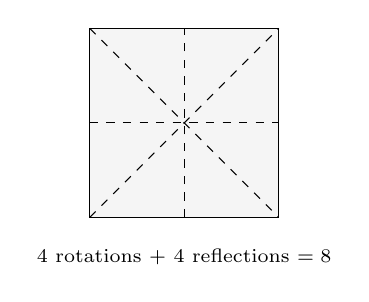
\begin{tikzpicture}[x=1mm,y=1mm]
  \draw[tile,fill=gray!8] (0,0) rectangle (24,24);
  \draw[dashed] (0,0) -- (24,24);
  \draw[dashed] (0,24) -- (24,0);
  \draw[dashed] (12,0) -- (12,24);
  \draw[dashed] (0,12) -- (24,12);
  \node[font=\scriptsize] at (12,-5) {$4$ rotations $+$ $4$ reflections $=8$};
\end{tikzpicture}
\end{center}

\noindent
Lean: \lean{lattice\_isometry\_cases} and \lean{isometry\_set\_eq} for the
classification, \lean{pointGroupSquare\_card} for the count $8$, and
\lean{pointGroupSquare\_rotations\_card} for the four rotations among them.

\section{Exam patterns: what to draw, and why it is a proof}

\begin{exercise}[Compute a determinant]
\emph{Draw} the parallelogram (or parallelepiped) spanned by the columns.  The
determinant is its signed area.  \emph{Why it is a proof:}
\lean{tile\_area\_eq\_abs\_det}.  Sanity check: two equal columns give a flat
tile, so the determinant is $0$.
\end{exercise}

\begin{exercise}[Row reduce, keeping track of the determinant]
\emph{Draw} the tile before and after.  Adding a multiple of a row shears it
(area unchanged), swapping rows reflects it (sign flips), scaling a row stretches
it.  \emph{Why:} \lean{row\_operation\_preserves\_det}, \lean{shear\_det}.
\end{exercise}

\begin{exercise}[$\det(AB) = \det A\,\det B$]
\emph{Draw} the unit tile, its image under $B$, and then under $A$.  Areas
multiply.  \emph{Why:} \lean{area\_scales\_by\_det} plus
\lean{det\_mul\_is\_retiling}.
\end{exercise}

\begin{exercise}[When is a system solvable, and what is the solution set?]
\emph{Draw} the domain striped by the parallel translates of $\ker A$.  If $b$
is in the image, the solutions form exactly one stripe: one particular solution
plus the kernel.  \emph{Why:} \lean{solution\_set\_is\_a\_tile},
\lean{fibre\_eq\_kernel\_translate}.
\end{exercise}

\begin{exercise}[Rank--nullity]
\emph{Draw} the same striped picture and count: the number of stripes is
$\dim\operatorname{im}$, the size of a stripe is $\dim\ker$.  \emph{Why:}
\lean{tiles\_times\_tile}.
\end{exercise}

\begin{exercise}[Show that a quantity is basis-independent]
\emph{Draw} the diagram without labels; anything you can read off is invariant.
For the trace, draw the closed loop and slide the boxes around it.
\emph{Why:} \lean{change\_of\_basis}; and \lean{Similar}, \lean{trace\_similar},
\lean{det\_similar}, \lean{charpoly\_similar} in \file{TraceLoop.lean}.
\end{exercise}

\begin{exercise}[Prove an identity about tensor/Kronecker products]
\emph{Draw} the two boxes side by side and slide one past the other.
\emph{Why:} \lean{interchange\_kronecker}, \lean{slide\_past\_wire}.
\end{exercise}

\begin{exercise}[Define a map and check it is well defined]
\emph{Draw} the triangle: a map out of a free module is a function on the basis.
\emph{Why:} \lean{unique\_extension\_from\_basis}.  For maps out of a
\emph{quotient}, the same triangle with the kernel condition:
\lean{quot\_triangle} in \file{CategoryDiagrams.lean}.
\end{exercise}

\begin{exercise}[Find all integer matrices of finite order / all lattice symmetries]
\emph{Draw} the lattice and ask which rotations map it to itself.
\emph{Why:} \lean{abs\_trace\_le\_two}, \lean{pow\_twelve\_eq\_one},
\lean{lattice\_isometry\_cases}.  Typical exam question: ``show that a finite
subgroup of $GL_2(\Z)$ has order dividing $24$'' --- the trace argument does it.
\end{exercise}

\section{Big ideas}

\begin{enumerate}
\item \textbf{Syntax is two-dimensional.}  A formula is a line of symbols and
  must invent brackets; a diagram is a graph and gets associativity, units and
  the interchange law for free.  What a string-diagram calculus buys is not new
  theorems but the elimination of bookkeeping.
\item \textbf{Every basic theorem is a normal-form statement.}  ``Every matrix
  is a product of elementary matrices'', ``every diagram equals a matrix in
  reduced form'', ``every morphism factors as epi followed by mono'': the same
  pattern, three languages.
\item \textbf{Invariance is the real content.}  Rank, trace, determinant and
  characteristic polynomial are the quantities that survive relabelling; in the
  diagram they are the features you can see without reading the labels.
\item \textbf{Relations, not just maps.}  Graphical linear algebra is
  \emph{not} the calculus of matrices: it is the calculus of linear relations,
  which is why boxes may be run backwards and why it has the extra
  copy/discard/add/zero generators.  Matrices are the sub-calculus of graphs of
  functions (\file{GraphicalLinearAlgebra.lean}, \file{DiagramDictionary.lean}).
\item \textbf{Counting is measuring is dimension.}  The determinant measures a
  tile, the rank counts tiles in the image, the index of a lattice in another
  lattice is again a determinant.  One idea, three names.
\item \textbf{Discreteness constrains symmetry.}  Integrality of the matrix of a
  symmetry plus boundedness of the trace of a rotation gives the
  crystallographic restriction.  A purely arithmetic fact ($2\cos\theta\in\Z$)
  rules out shapes.
\item \textbf{The same proof appears at three levels.}  The proof that the
  trace is conjugation invariant, the proof that a closed wire may be slid, and
  the dinaturality of the categorical trace are literally the same argument in
  three notations.
\end{enumerate}

\section{Cool facts}

\begin{itemize}
\item \textbf{No fivefold symmetry.}  A unimodular integer $2\times2$ matrix
  with $A^5=I$ is the identity (\lean{no\_fivefold\_symmetry}); yet
  quasi-periodic Penrose tilings do have fivefold symmetry in a weaker,
  non-crystallographic sense --- the theorem forbids exact translational
  periodicity, not the pattern.
\item \textbf{Sixfold is attained.} $\left(\begin{smallmatrix}0&-1\\1&1
  \end{smallmatrix}\right)$ has order exactly $6$
  (\lean{hexagonal\_rotation\_pow\_six}, and its cube and square are not the
  identity).
\item \textbf{Order twelve.} Every finite-order element of $SL_2(\Z)$ satisfies
  $A^{12}=I$ (\lean{pow\_twelve\_eq\_one}).
\item \textbf{The trace of a rotation is $2\cos\theta$}, so a rotation of a
  lattice has $2\cos\theta\in\{0,\pm1,\pm2\}$: the entire classification of
  wallpaper rotation orders is one integrality argument
  (\lean{cos\_of\_lattice\_rotation}).
\item \textbf{Cayley--Hamilton in size two is a one-line computation}
  ($A^2 = (\tr A)A - (\det A)I$, \lean{cayley\_hamilton\_two}) and it powers the
  whole crystallographic argument through the trace recursion
  $s_{k+2} = t s_{k+1} - s_k$ (\lean{trace\_pow\_rec}) --- the same recursion
  that produces Chebyshev polynomials and Fibonacci-like growth.
\item \textbf{The square lattice has exactly $8$ symmetries, the ``generic''
  lattice exactly $2$} ($\pm I$): symmetry is the exception
  (\lean{pointGroupSquare\_card}).
\item \textbf{A shear is invisible to area} but not to shape: Cavalieri's
  principle and the invariance of the determinant under row operations are the
  same statement (\lean{shear\_preserves\_area}).
\item \textbf{Cutting a wire is a partition of unity.}  $\sum_i E_{ii} = I$ is
  the smallest tiling in mathematics (\lean{identity\_is\_tiled}).
\item \textbf{Bending a wire twice does nothing} --- the snake equation --- and
  that is the entire reason $(A^{\!\top})^{\!\top} = A$ and
  $(AB)^{\!\top}=B^{\!\top}A^{\!\top}$ (\lean{bend\_twice},
  \lean{bend\_series}).
\end{itemize}

\section{What is formalised, and where}

\begin{center}\small
\begin{tabular}{@{}p{52mm}p{95mm}@{}}
\toprule
\textbf{file} & \textbf{contents} \\
\midrule
\file{CommonPatterns.lean} & the eight shared patterns: composition, functoriality of
  \lean{toMatrix}, interchange (products and Kronecker), unique extension from a
  basis, bending a wire, partitions of the identity, change of basis, and the
  fibre tiling with rank--nullity \\
\file{Tilings.lean} & lattice tilings and fundamental domains, area
  $=|\det|$, the determinant as area scale factor, shears and row operations,
  the crystallographic restriction (algebraic and geometric form), no fivefold
  symmetry, the order-$6$ witness, and the point group of the square lattice \\
\file{GraphicalLinearAlgebra.lean}, \file{DiagramDictionary.lean} & diagrams as
  linear relations, and the dictionary to matrices and Penrose notation \\
\file{SzaboFields.lean}, \file{SzaboMatrices.lean}, \file{SzaboDeterminant.lean} &
  the textbook layer: number fields, matrices, the recursive determinant \\
\file{CategoryDiagrams.lean}, \file{ExistentialGraphs.lean} & commutative-diagram
  proofs; Peirce's alpha graphs \\
\file{ExamPatterns.lean}, \file{TraceLoop.lean} & standard exam patterns; the
  trace as a closed wire \\
\bottomrule
\end{tabular}
\end{center}

\noindent
Build with \lean{lake build}; rebuild this note with \lean{tectonic patterns.tex}.

\begin{thebibliography}{9}
\bibitem{gs} B.~Grünbaum and G.~C.~Shephard, \emph{Tilings and Patterns},
  Freeman, 1987.
\bibitem{maclane} S.~Mac Lane, \emph{Categories for the Working Mathematician},
  2nd ed., Springer.
\bibitem{szabo} L.~Szabó, \emph{Bevezetés a lineáris algebrába}, Polygon,
  Szeged, 2006.
\bibitem{gla} P.~Sobociński, \emph{Graphical Linear Algebra},
  \url{https://graphicallinearalgebra.net}.
\end{thebibliography}

\end{document}
